\documentclass{article}
\usepackage[usenames,dvipsnames,svgnames]{xcolor}
\usepackage[utf8]{inputenc}
\usepackage{algpseudocode}
\usepackage{amsfonts}
\usepackage{amsmath}
\usepackage{amssymb}
\usepackage{amsthm}
\usepackage{algorithm}
\usepackage{tikz}
\usepackage{subcaption}
\usepackage{fancyvrb}
\usepackage{bm}
\usepackage{textcomp}
\usepackage{listings}
\usepackage{todonotes}
\usepackage{mathtools} % long right arrow
\usepackage{proof} % for infer
\usepackage{setspace} % set line spacing
\usepackage{amsthm}

\newtheorem{theorem}{Theorem}[section]
\newtheorem{corollary}{Corollary}[theorem]
\newtheorem{lemma}[theorem]{Lemma}
\newtheorem{definition}{Definition}[section]

\newcommand{\code}[1]{\texttt{\small{\textbf{#1}}}}
\newcommand{\reals}[0]{\mathbb{R}}
\newcommand{\naturals}[0]{\mathbb{N}}
\newcommand{\integers}[0]{\mathbb{Z}}
\newcommand{\rationals}[0]{\mathbb{Q}}
\newcommand\doubleplus{\mathbin{+\mkern-5mu+}}
\newcommand{\concat}[0]{\doubleplus}
\newcommand{\diff}[0]{\setminus}
\newcommand{\dom}[1]{\mbox{dom}{~#1}}
\newcommand{\emptytrace}[0]{\epsilon}
\newcommand{\gen}[0]{\mbox{\scriptsize gen}}
\newcommand{\force}[0]{\mbox{\scriptsize force}}
\newcommand{\fix}[0]{\mbox{\scriptsize fix}}
\newcommand{\contained}[0]{\sqsubseteq}

% coordinates for tikz address schematics
\newcommand{\innerll}[0]{(0.25 + 0.625, 0.625)}
\newcommand{\innerlr}[0]{(0.25 + 0.625 + 0.5, 0.625)}
\newcommand{\innerur}[0]{(0.25 + 0.625 + 0.5, 0.625 + 0.5)}
\newcommand{\innerul}[0]{(0.25 + 0.625, 0.625 + 0.5)}
\newcommand{\outerll}[0]{(0.25, 0)}
\newcommand{\outerlr}[0]{(0.25 + 1.75, 0)}
\newcommand{\outerur}[0]{(0.25 + 1.75, 1.75)}
\newcommand{\outerul}[0]{(0.25, 1.75)}
\newcommand{\all}[0]{(0, 0)}
\newcommand{\alr}[0]{(2, 0)}
\newcommand{\aur}[0]{(2, 2)}
\newcommand{\aul}[0]{(0, 2)}
\newcommand{\bll}[0]{(0.25, -0.25)}
\newcommand{\blr}[0]{(2.25, -0.25)}
\newcommand{\bur}[0]{(2.25, 1.75)}
\newcommand{\bul}[0]{(0.25, 1.75)}

\title{Gen Semantics}
\author{Marco Cusumano-Towner}

\begin{document}

\maketitle

\section{Traces}
A \emph{trace} is a finite map from \emph{addresses} to \emph{values}, which for simplicity, we assume are elements of some finite set $V$.
The `set of addresses' in a trace $t$ is its domain $\dom{t}$.
For traces $s$ and $t$ with disjoint domains $\dom{s}$ and $\dom{t}$, let $u = s \concat t$ denote the trace $u$ with $\dom{u} = \dom{s} \cup \dom{t}$ and $u(a) = s(a)$ for $a \in \dom{s}$ and $u(a) = t(a)$ for $a \in \dom{t}$.
For two traces $s$ and $t$, let $s \contained t$ denote the relation that $\dom{s} \subseteq \dom{t}$ and that $s(a) = t(a)$ for all $a \in \dom{s}$ ($s$ is a restriction of $t$).
For $s \contained t$, let $u = t \diff s$ denote the trace with $u(a) = s(a)$ for each $a \in \dom{t} \setminus \dom{s}$.
Let $t|_S$ denote the restriction of a trace $t$ to a set $S$ of addresses, so that $\dom{t|_S} = \dom{t} \cap S$.
Let $\emptytrace$ denote the empty trace (with $\dom \emptytrace = \varnothing$).

\section{Probabilistic Module}
A \emph{probabilistic module} is a tuple $(X, p, U, q_{gen}, q_{fix}, q_{free}, \theta, f)$, where $X$ is the set of valid \emph{inputs} to the module, and where $p$, $q_{gen}$ and $q_{fix}$, $q_{free}$ are indexed sets of probability distribution on traces, where $\theta$ are current parameters of the module (upon which $p$ has an implicit dependence).
Specifically, $p(t; x) \ge 0$ where $t$ is a trace, and where $x \in X$ and $\sum_t p(t; x) = 1$ for all $x \in X$.
$p(t; x)$ is the probability of a trace given input $x$.
Let $T_x = \{t : p(t; x) > 0 \}$ denote the set of \emph{possible traces} for input $x \in X$.
The function $f : \{(x, t) : x \in X, t \in T_x\} \to Y$ defines the \emph{output value} $y \in Y$ given the inputs and a trace.

We require that $p$ satisfies the following \emph{well-behaved addresses property}:
For all $x \in X$ and all $s, t \in T_x$, if $\dom{s} \ne \dom{t}$ then $\exists a \in \dom{s} \cap \dom{t}$ such that $s(a) \ne t(a)$.
In words, different address sets for the same arguments $x$ must be explained by different value{s} for some shared address(es).


% TODO all of the methods will accept arbitary configuration, which is
% recursively dispatched throughout the call hierarchy during calls to methods.
% the address selection is one example type of configuration used to configure
% free_update.

\paragraph{Generate Method (\code{generate})}
For each $x \in X$, let $U^{gen}_x$ denote a set of traces, called \emph{valid generation constraints}, such that for each $u \in U^{\gen}_x$ there exists some $t \in T_x$ where $u \contained t$.
$U^{\gen}_x$ need not include all such $u$ (i.e. $U^{\gen}_x$ is not necessarily the set of all projections of all traces in $T_x$).
We require that $\emptytrace \in U^{\gen}_x$.
Then, for each $x \in X$ and $u \in U^{\gen}_x$, we require that $q_{\gen}(s; u, x) > 0$ if and only if $t = s \concat u$ for some $t \in T_x$.
We also require that $\sum_s q_{\gen}(s; u, x) = 1$.
Given $x \in X$ and $u \in U^{\gen}_x$, sample $s \sim q_{\gen}(\cdot; u, x)$, and return $t = s \concat u$ and a weight $p(t; x) / q(s; u, x)$.
Also return $y = f(x, t)$.

%% generate address schematic %%
\begin{figure}[t]
\centering
% dom t
\begin{subfigure}[b]{0.3\textwidth}
\centering
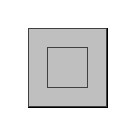
\begin{tikzpicture}
\draw (0, 0) rectangle (1, 1);
\draw (0.25, 0.25) rectangle (0.75, 0.75);
\filldraw [gray, fill opacity=0.5, draw opacity=0.0] (0, 0) -- (0, 1) -- (1, 1) -- (1, 0);
\end{tikzpicture}
\caption{$\dom{t}$}
\end{subfigure}%
% dom u
\begin{subfigure}[b]{0.3\textwidth}
\centering
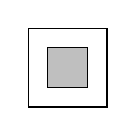
\begin{tikzpicture}
\draw (0, 0) rectangle (1, 1);
\draw (0.25, 0.25) rectangle (0.75, 0.75);
\filldraw [gray, fill opacity=0.5, draw opacity=0.0] (0.25, 0.25) -- (0.25, 0.75) -- (0.75, 0.75) -- (0.75, 0.25);
\end{tikzpicture}
\caption{$\dom{u}$}
\end{subfigure}
% dom s
\begin{subfigure}[b]{0.3\textwidth}
\centering
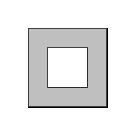
\begin{tikzpicture}
\draw (0, 0) rectangle (1, 1);
\draw (0.25, 0.25) rectangle (0.75, 0.75);
\filldraw [gray, fill opacity=0.5, draw opacity=0.0] (0, 0) -- (1, 0) -- (1, 1) -- (0, 1) (0.25, 0.25) -- (0.25, 0.75) -- (0.75, 0.75) -- (0.75, 0.25);
\end{tikzpicture}
\caption{$\dom{s}$}
\end{subfigure}
\caption{Schematic showing addresses of traces involved in \code{generate}}
\end{figure}

\paragraph{Force Update Method (\code{force\_update})}
For $x, x' \in X$, and $t \in T_x$, let $U^{\force}_{x,x',t}$ denote the set of traces $u$ such that there exists $t' \in T_{x'}$ where $u \contained t'$ and $\{ a: t(a) \ne t'(a)\} \subseteq \dom{u}$, and $\dom{t'} \setminus \dom{t} \subseteq \dom{u}$.
That is, $u$ contains values for at least all addresses that differ between $t$ and $t'$, and all addresses in $t'$ that are not in $t$.
Return $t'$ (see Lemma~\ref{lemma:force-update-unique} for uniqueness of $t'$), and the weight $p(t'; x') / p(t; x)$ and $y = f(x', t')$.
Also return the \emph{discard trace} $v$ given by $v(a) = t(a)$ for $a \in (\dom{t'} \setminus \dom{t}) \cup (\dom{t} \cap \dom{u})$.

\begin{lemma} \label{lemma:force-update-unique}
For any such $x, x', t, u$, the trace $t'$ is unique.
\end{lemma}
\begin{proof}
Suppose there exists $t'_1 \ne t'_2$ such that $u \contained t'_1$ and $u \contained t'_2$ and such that $\dom{u} \supseteq \{a : t(a) \ne t'_1(a) \lor t(a) \ne t'_2(a)\} \cup ((\dom{t'_1} \cup \dom{t'_2}) \setminus \dom{t})$.
If $\dom{t'_1} = \dom{t'_2}$ then there must be an address $b$ such that $t'_1(b) \ne t(b)$ or $t'_2(b) \ne t(b)$, which implies $b \in \dom{u}$, which implies $t'_1(b) = t'_2(b) = u(b)$, which is a contradiction.
If $\dom{t'_1} \ne \dom{t'_2}$, then by the well-behaved address property, there must be an address $b$ such that $t'_1(b) \ne t'_2(b)$, which implies $b \in \dom{u}$, which implies $t'_1(b) = t'_2(b) = u(b)$, which is a contradiction.
\end{proof}

%% force update address schematic %%
\begin{figure}[t]
\centering
% dom t
\begin{subfigure}[b]{0.2\textwidth}
\centering
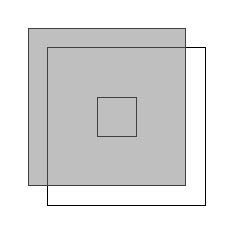
\begin{tikzpicture}
\draw \all{} rectangle \aur{};
\draw \bll{} rectangle \bur{};
\draw \innerll{} rectangle \innerur{};
\filldraw [gray, fill opacity=0.5, draw opacity=0.0] \all{} -- \alr{} -- \aur{} -- \aul{};
\end{tikzpicture}
\caption{$\dom{t}$}
\end{subfigure}%
% dom t'
\begin{subfigure}[b]{0.2\textwidth}
\centering
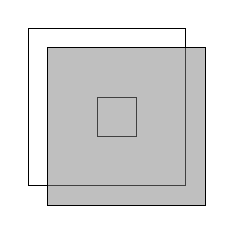
\begin{tikzpicture}
\draw \all{} rectangle \aur{};
\draw \bll{} rectangle \bur{};
\draw \innerll{} rectangle \innerur{};
\filldraw [gray, fill opacity=0.5, draw opacity=0.0] \bll{} -- \blr{} -- \bur{} -- \bul{};
\end{tikzpicture}
\caption{$\dom{t'}$}
\end{subfigure}%
% dom u
\begin{subfigure}[b]{0.2\textwidth}
\centering
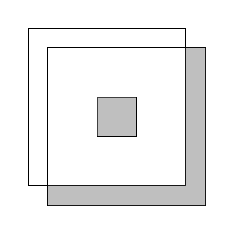
\begin{tikzpicture}
\draw \all{} rectangle \aur{};
\draw \bll{} rectangle \bur{};
\draw \innerll{} rectangle \innerur{};
\filldraw [gray, fill opacity=0.5, draw opacity=0.0] \innerll{} -- \innerlr{} -- \innerur{} -- \innerul{};
\filldraw [gray, fill opacity=0.5, draw opacity=0.0] \outerll{} -- \outerlr{} -- \outerur{} -- \bur{} -- \blr{} -- \bll{} -- \outerll{};
\end{tikzpicture}
\caption{$\dom{u}$}
\end{subfigure}%
% dom v
\begin{subfigure}[b]{0.2\textwidth}
\centering
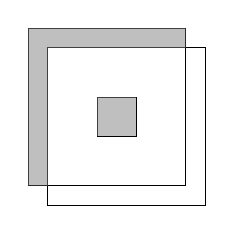
\begin{tikzpicture}
\draw \all{} rectangle \aur{};
\draw \bll{} rectangle \bur{};
\draw \innerll{} rectangle \innerur{};
\filldraw [gray, fill opacity=0.5, draw opacity=0.0] \innerll{} -- \innerlr{} -- \innerur{} -- \innerul{};
\filldraw [gray, fill opacity=0.5, draw opacity=0.0] \outerll{} -- \outerul{} -- \outerur{} -- \aur{} -- \aul{} -- \all{} -- \outerll{};
\end{tikzpicture}
\caption{$\dom{v}$}
\end{subfigure}%
% dom r
\begin{subfigure}[b]{0.2\textwidth}
\centering
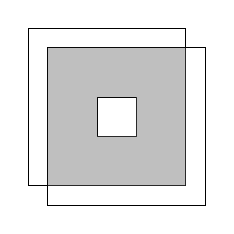
\begin{tikzpicture}
\draw \all{} rectangle \aur{};
\draw \bll{} rectangle \bur{};
\draw \innerll{} rectangle \innerur{};
\filldraw [gray, fill opacity=0.5, draw opacity=0.0] \outerll{} -- \outerlr{} -- \outerur{} -- \outerul{} \innerll{} -- \innerul{} -- \innerur{} -- \innerlr{};
\end{tikzpicture}
\caption{$\dom{r}$}
\end{subfigure}
\caption{Schematic showing addresses of traces involved in \code{force\_update}}
\end{figure}

\paragraph{Fix Update Method (\code{fix\_update})}
For $x, x' \in X$ and $t \in T_x$, let $U^{\fix}_{x,x',t}$ denote the set of traces $u$ such that $\dom{u} \subseteq \dom{t}$ and such that there exists traces $s$ and $r$ with $\dom{s} \cap \dom{t} = \varnothing$, $\dom{r} \subseteq \dom{t}$, $\dom{r} \cap \dom{u} = \varnothing$ where $u \concat s \concat r \in T_{x'}$.
For each $x, x' \in X$, $t \in T_x$, and $u \in U^{\fix}_{x,x',t}$, there is a probability distribution on traces $s$, denoted $q_{\fix}(s; x, x', t, u)$, such that $q_{\fix}(s; x, x', t, u) > 0$ if and only if there exists a trace $r$ with $\dom{r} \subseteq \dom{t}$ and $\dom{r} \cap \dom{u} = \varnothing$ where $t' = u \concat s \concat r \in T_{x'}$.

\begin{lemma} \label{lemma:fix-update-unique}
For any such $x, x', t, u, s$, the traces $r$ and $t'$ are unique.
\end{lemma}
\begin{proof}
\end{proof}

Given $x, x' \in X, t \in T_x, u \in U^{\fix}_{x,x',t}$, sample $s \sim q_{\fix}(\cdot; x, x', t, u)$ and return $t' = u \concat s \concat r$, the \emph{discard trace} $v$ where $v(a) = t(a)$ for $a \in \dom{u}$, and the weight:
\[
\frac{p(t'; x')}{p(t; x)} \frac{q_{\fix}(s'; x', x, t', v)}{q_{\fix}(s; x, x', t, u)}
\]
where $s' = t|_{\dom{t} \setminus \dom{t'}}$ contains the part of $t$ that was \emph{deleted}.
Also return $y = f(x', t')$.

\begin{lemma} \label{lemma:fix-update-reverse}
If $x, x' \in X, t \in T_x, u \in U^{\fix}_{x, x', t}$, and $s$ where $q_{\fix}(s; x, x', t, u) > 0$, $v \in U^{\fix}_{x',x,t'}$ and $q^{\fix}(s'; x', x, t') > 0$, then $v \concat s' \concat r' = t$ for $r'(a) = t(a)$ for $a \in (\dom{t} \cap \dom{t'}) \setminus \dom{u}$.
\end{lemma}
\begin{proof}
\end{proof}


\paragraph{Free Update Method (\code{free\_update})}
Given $x, x' \in X$, and $t \in T_x$, $q_{free}(t'; t, x, x')$ is a distribution on traces such that $q_{free}(t'; t, x, x') > 0$ implies $t' \in T_{x'}$, and such that $q_{free}(t'; t, x, x') > 0$ implies $q_{free}(t; t', x', x) > 0$.
Sample $t' \sim q_{free}(\cdot; t, x, x')$ and return $t'$, and a weight:
\[
    \frac{p(t'; x')}{p(t; x)} \frac{q_{free}(t; t', x', x)}{q_{free}(t'; t, x, x')}
\]
Also return $y' = f(x', t')$.
Note that `regenerate', where we provide a set of addresses that should be resimulated, is an example of this.

\paragraph{Backpropagate to Parameters Method (\code{backprop\_params})}
Given $x \in X$ and $t \in T_x$, and $\nabla_y J$, return $\nabla_x (J + \log p(t; x))$ and $\nabla_{\theta} (J + \log p(t; x))$.

% \paragraph{Backpropagate to Trace (\code{backprop\_trace})}
% TODO doesn't make sense if values come from a discrete set

Each probabilistic module may also possess an indexed collection of families of distributions for use in \code{generate} and \code{update}.
Probabilistic modules may also have update procedures that make arbitrary changes to their trace, and return the appropriate weight.
These two features are not yet implemented.

\section{Untraced Random Choices}

\section{Generative Functions}
% an example of a probabilistic module that is composed of other probabilistic modules.
% give implementations of these various things (as small step semantics?)

\clearpage
\bibliographystyle{abbrv}
\bibliography{references}

\end{document}
